% Dieses Dokument dient als Cheatsheet für verschiedene Technologien in LaTeX, die ich benutze.
% Ich erhebe keinen Anspruch auf Vollständigkeit und Best Practices
\documentclass[10pt,a4paper]{article}

\usepackage{mystyle}
\usepackage{hyperref} 

\begin{document}
% Titel einbinden
% Titelseite
\pagenumbering{gobble}
\maketitle
\newpage
\pagenumbering{Roman}
% Inhaltsverzeichnis, Bildverzeichnis, Tabellenverzeichnis
\tableofcontents
\newpage
\listoffigures
\newpage
\listoftables
\newpage
\pagenumbering{arabic}

% Listen-Datei einbinden
% Listenbeispiel
\section{Listenbeispiel}
    \begin{itemize}
        \item One entry in the list
        \item Another entry in the list
    \end{itemize}
    \begin{enumerate}
        \item One entry in the list
        \item Another entry in the list
    \end{enumerate}

% Tabellen-Datei einbinden
% Tabellenbeispiel
% Mehr Infos unter https://www.overleaf.com/learn/latex/Tables
\section{Tabellenbeispiel}
\begin{table}[h]
    \begin{tabularx}{\textwidth}{|l|X|c|r|}
        \hline
        \textbf{Nr.} & \textbf{Beschreibung} & &\\
        \hline
        1. & Ich schreibe lange Texte, um meinen Standpunkt 
        zu verdeutlicheStandpStandpunkt zu verdeutlichenunkt 
        zu verdeutlichenn  & schrift  &  123 \\
        \hline
        2. & Ich schreibe lange Texte, um meinen Standpunkt 
        zu verdeutlichen  & Schr  &   1234567 \\
        \hline
        3. & Ich schreibe lange Texte, um meinen Standpunkt
        & Schriftift  &   12 \\
        \hline
        4. & Ich schreibe lange Texte, um meinen Standpunkt 
        zu verdeutlichen  &   &   1234 \\
        \hline
    \end{tabularx}
    \caption{Beispieltabelle}
\label{tab:Beispieltabelle}
\end{table}
    

% Bildbeispiel einbinden
% Bildbeispiel einbinden
% Weiteres findest du unter https://de.overleaf.com/learn/latex/Inserting_Images
\section{Beispielbild}
\begin{figure}[h]
    \centering
    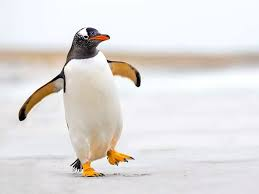
\includegraphics[width=0.75\linewidth]{penguin}
    \caption{Eselspinguin}
    \label{fig:penguin}
\end{figure}

% Beispiel für Referenzierung
% Hier ein paar Beispielreferenzen
\section{Referenzenbeispiel}
Hier findest du das Pinguin-Bild \ref{fig:penguin}.
Hier findest du das Tikz-Beispiel \ref{fig:Tikzbeispiel}.
Hier findest du die Beispieltabelle \ref{tab:Beispieltabelle}.

\end{document}